\section{Pieczona fasolka szparagowa}
\bigskip
\small
\begin{minipage}{0.45\textwidth}
    \noindent \textbf{Czas:} 45 minut \\
    \textbf{Poziom trudności:} łatwy
\end{minipage}
\begin{minipage}{0.45\textwidth}
    \noindent \textbf{Ilość sprzątania:} średnia\\
    \textbf{Wymagany mysi sprzęt:} piekarnik
\end{minipage}
\normalsize
\vspace{0.5cm}

\begin{multicols}{2}

\subsection*{Składniki}
\begin{itemize}
    \item szczodra garść fasolki szparagowej
    \item 1 łyżeczka skórki z limonki
    \item 3 łyżki orzeszków ziemnych
    \item 4 łyżki oliwy
    \item 0.25 łyżeczki płatków chilli lub pieprzu cayenne
    \item mała garstka świeżej kolendry (można zastąpić listkami bazylii, mięty, lub pietruszki)
    \item sól do smaku
\end{itemize}

\columnbreak

\begin{figure}[H]
    \centering
    \fbox{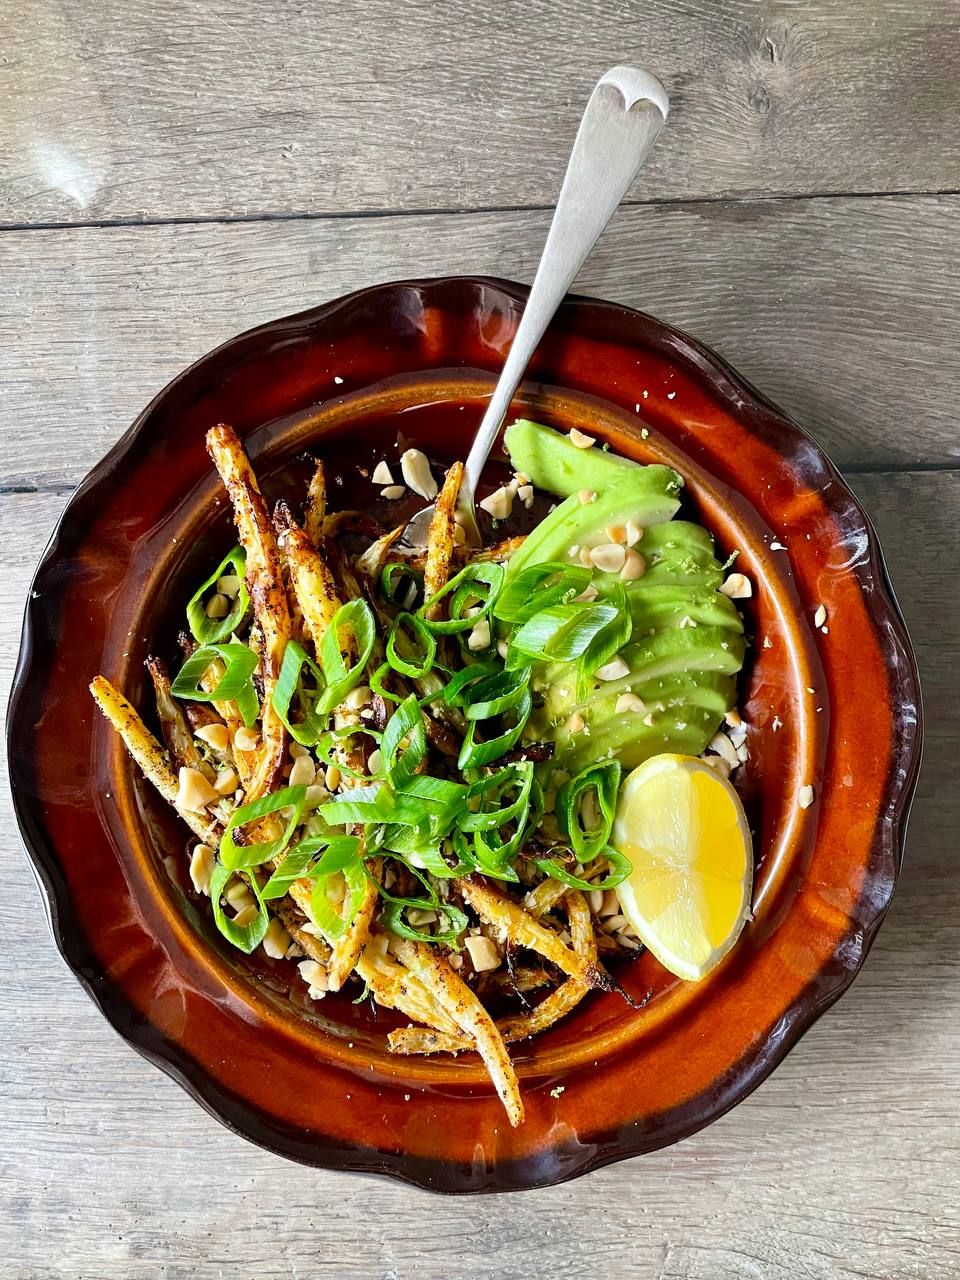
\includegraphics[width=0.35\textwidth]{images/fasolka-szparagowa.jpg}}
\end{figure}
\end{multicols}

\vspace{0.5cm}

\subsection*{Instruktaż}
\begin{enumerate}
    \item Piekarnik rozgrzać do 220 stopni Celsjusza i blaszkę wyłożyć papierem do pieczenia
    \item Odciąć zdrewniałe końcówki z fasolki szparagowej i przełożyć na blaszkę wraz z skórką z limonki, chili oraz hojną szczyptą soli. Skropić oliwą i dokładnie obtoczyć fasolkę w marynacie – najlepiej rękami.
    \item Piec przez 30 – 40 minut, aż fasolka będzie miękka i częściowo poczernieje na brzegach.
    \item Po upieczeniu dodać orzeszki ziemne oraz kolendrę i dokładnie wymieszać.
\end{enumerate}

\vspace{0.5cm}

\small
\subsection*{Propozycja podania}
Ze świeżym sokiem z limonki, z bułką tartą podsmażoną na maśle, z awokado, jako dodatek do obiadu.

\vspace{0.3cm}

\subsection*{Dodatkowe uwagi}
Fasolkę najlepiej podawać zaraz po upieczeniu, aby nie traciła na chrupkości.

\newpage
